\section{Principe du maillon faible}

\subsection{Pr�sentation du principe}

\begin{frame}
  \frametitle{Principe du maillon faible}

  \begin{columns}
    \begin{column}{0.7\textwidth}<1->
      \begin{itemize}
      \item<1-> La s�curit� d'un syst�me est celle de l'�l�ment le plus faible. 
      \item<2-> Il faut connaitre tous les �l�ments du syst�me, ne rien n�gliger.
      \item<3-> Rien ne sert d'installer une porte blind�e sur un mur en carton. 
      \end{itemize}
    \end{column}
  \end{columns}
\end{frame}

\subsection{Exemple : Authentification sur un ordinateur (local)}

\begin{frame}
  \frametitle{Exemple : Authentification sur un ordinateur (local)}

  \begin{columns}
    \begin{column}{0.7\textwidth}<1->
      \begin{itemize}
      \item<1-> Choix des mots de passe.
      \item<2-> Est-ce que le bootloader (Lilo/Grub) est s�curis� ? 
      \item<3-> Est-ce que le BIOS est s�curis� ?
      \item<4-> Est-ce que l'ordinateur est physiquement s�curis� ?\\
      (ferm� par un cadenas et attach� au bureau)
      \end{itemize}
    \end{column}
  \end{columns}
\end{frame}

\subsection{Exemple : Faille dans Linux}

\begin{frame}[t]
  \frametitle{Exemple : Faille dans Linux}
  \framesubtitle{Architecture d'un ordinateur}

  \begin{columns}
    \begin{column}{0.7\textwidth}<1->
    \begin{itemize}
      \item<1-> Applications : Firefox, Gimp, Gvim, Xchat, etc.
      \item<2-> Biblioth�ques : libc, zlib, GTK, X11, etc.
      \item<3-> Noyau : Linux, OpenBSD, Hurd, etc.
      \item<4-> Mat�riel : Processeur, m�moire, carte vid�o, chipset, etc.
    \end{itemize}    
    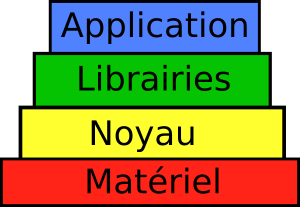
\includegraphics[height=10ex]{schema_appli.eps}
    \end{column}
  \end{columns}
\end{frame}

\begin{frame}
  \frametitle{Exemple : Faille dans Linux}
  \framesubtitle{Faille chown}

  \begin{columns}
    \begin{column}{0.7\textwidth}<1->
      \begin{itemize}
      \item<1-> Linux est d�velopp� par des humains, et du coup est
      faillible. Des failles sont r�guli�rement d�couvertes dans le
      noyau.
      \item<2-> Exemple : faille permettant de changer le propri�taire 
      (groupe) d'un fichier dans les version inf�rieures � 2.4.28 et
      2.6.8. Voir l'exploit :
      www.0xdeadbeef.info/exploits/raptor\_chown.c
      \end{itemize}
    \end{column}
  \end{columns}
\end{frame}

\begin{frame}
  \frametitle{Exemple : Faille dans Linux}
  \framesubtitle{Extrait de l'exploit chown}

  \begin{center}
     chown(argv[1], -1, getgid());

     \begin{itemize}
       \item argv[1] : Nom du fichier
       \item -1 : Propri�taire du fichier, -1 signifie "pas de changement"
       \item getgid() : Groupe du fichier, utilise le groupe de l'utilisateur
       ayant lanc� le programme.
     \end{itemize}
  \end{center}
\end{frame}


